% \documentclass[a4paper,11pt,twoside,class=meetingmins,crop=false,agenda]{standalone}
% \documentclass[a4paper,11pt,twoside,class=meetingmins,crop=false,chair]{standalone}
\documentclass[a4paper,11pt,twoside,class=meetingmins,crop=false]{standalone}
\newcommand{\meetingType}{board}
\usepackage{groupmeetings}

\begin{document}

\setdate{2016--01--13}
\setpresent{
    \chair{A.~Goodsell},
    \boardmember{M.~Fry},
    L.~Foglianti Spadini,
    A.~Hyslop,
    A.~Kallaivannan,
    R.~Kent,
    C.~Lau,
    A.~Rutley,
    S.~Searles-Bryant,
    S.~Wright,
    L.~Yeo
}

\maketitle

\section{Announcements}
\begin{hiddenitems}
    \item
    The assessment criteria for the peer-assessment component of the module have been chosen:
    \begin{description}
        \item[Communication] ``Exchanging ideas and updating others on progress/feedback.''
        \item[Productivity] ``Maximising your contribution within a given time frame.''
        \item[Participation] ``Willingness to engage in, and contribute to, the project.''
        \item[Quality] ``Clear work which significantly furthers the progress of the project.''
        \item[Cooperation] ``Prioritising effectively towards a common goal.''
        \item[Reliability] ``Do what you say you're going to do; be trustworthy.''
    \end{description}
    Scores should be between 1 and 3 (less than expected; expected; exceeds expectations).
    These must be sent weekly to MF before 17.00 each Monday, starting Monday, January 25.

\end{hiddenitems}

\section{Allocation of roles}
\begin{items}
    \item AG will chair meeting and act as the team leader.
    \item SSB will take minutes and act as the contact person for MF and the course coordinator.
    \item RK will collate the peer-assessment scores and send to SSB to forward to MF each week.
    \item CL will act as the group treasurer.
\end{items}

\section{Project brief (MF)}
% Project brief document attached.
\begin{quotation}
``The challenge is to develop a robot which can draw artwork on sandy beaches.''
\end{quotation}
\begin{hiddenitems}
    \item The final product should be small enough to fit in a rucksack/suitcase. It should be manageable on public transport.
    \item Examples of sand art at \url{https://www.flickr.com/photos/martinartman}.
    \item The product can draw large-scale on a beach, or small-scale in a table-top sandpit.
    \item The robot should be named
    \item The specifics of what sorts of images the robot should draw are left for us to decide; the purpose and motivations for the project have not been specified.
\end{hiddenitems}

\section{Resources}
\begin{hiddenitems}
    \item The project budget is \pounds{200}.
    \item A case can be made to the course coordinator to obtain extra funding (MF advises probably only up to \textsterling50).
    \item The robot designed for this course a few years ago is available for parts. MF advises that the motors (value c. \pounds{100}) are particularly useful.
\end{hiddenitems}

\vspace{1em}
\nextmeeting{Tuesday, January 19, at 11:15 in MPEB 3.14a}
\vspace{1em}

\section{Actions}
\begin{items}
    \action{Discuss skills and divide responsibilities among team members}{all}
    \action{Decide upon purpose and motivations for the product}{all}
\end{items}
% \newpage
%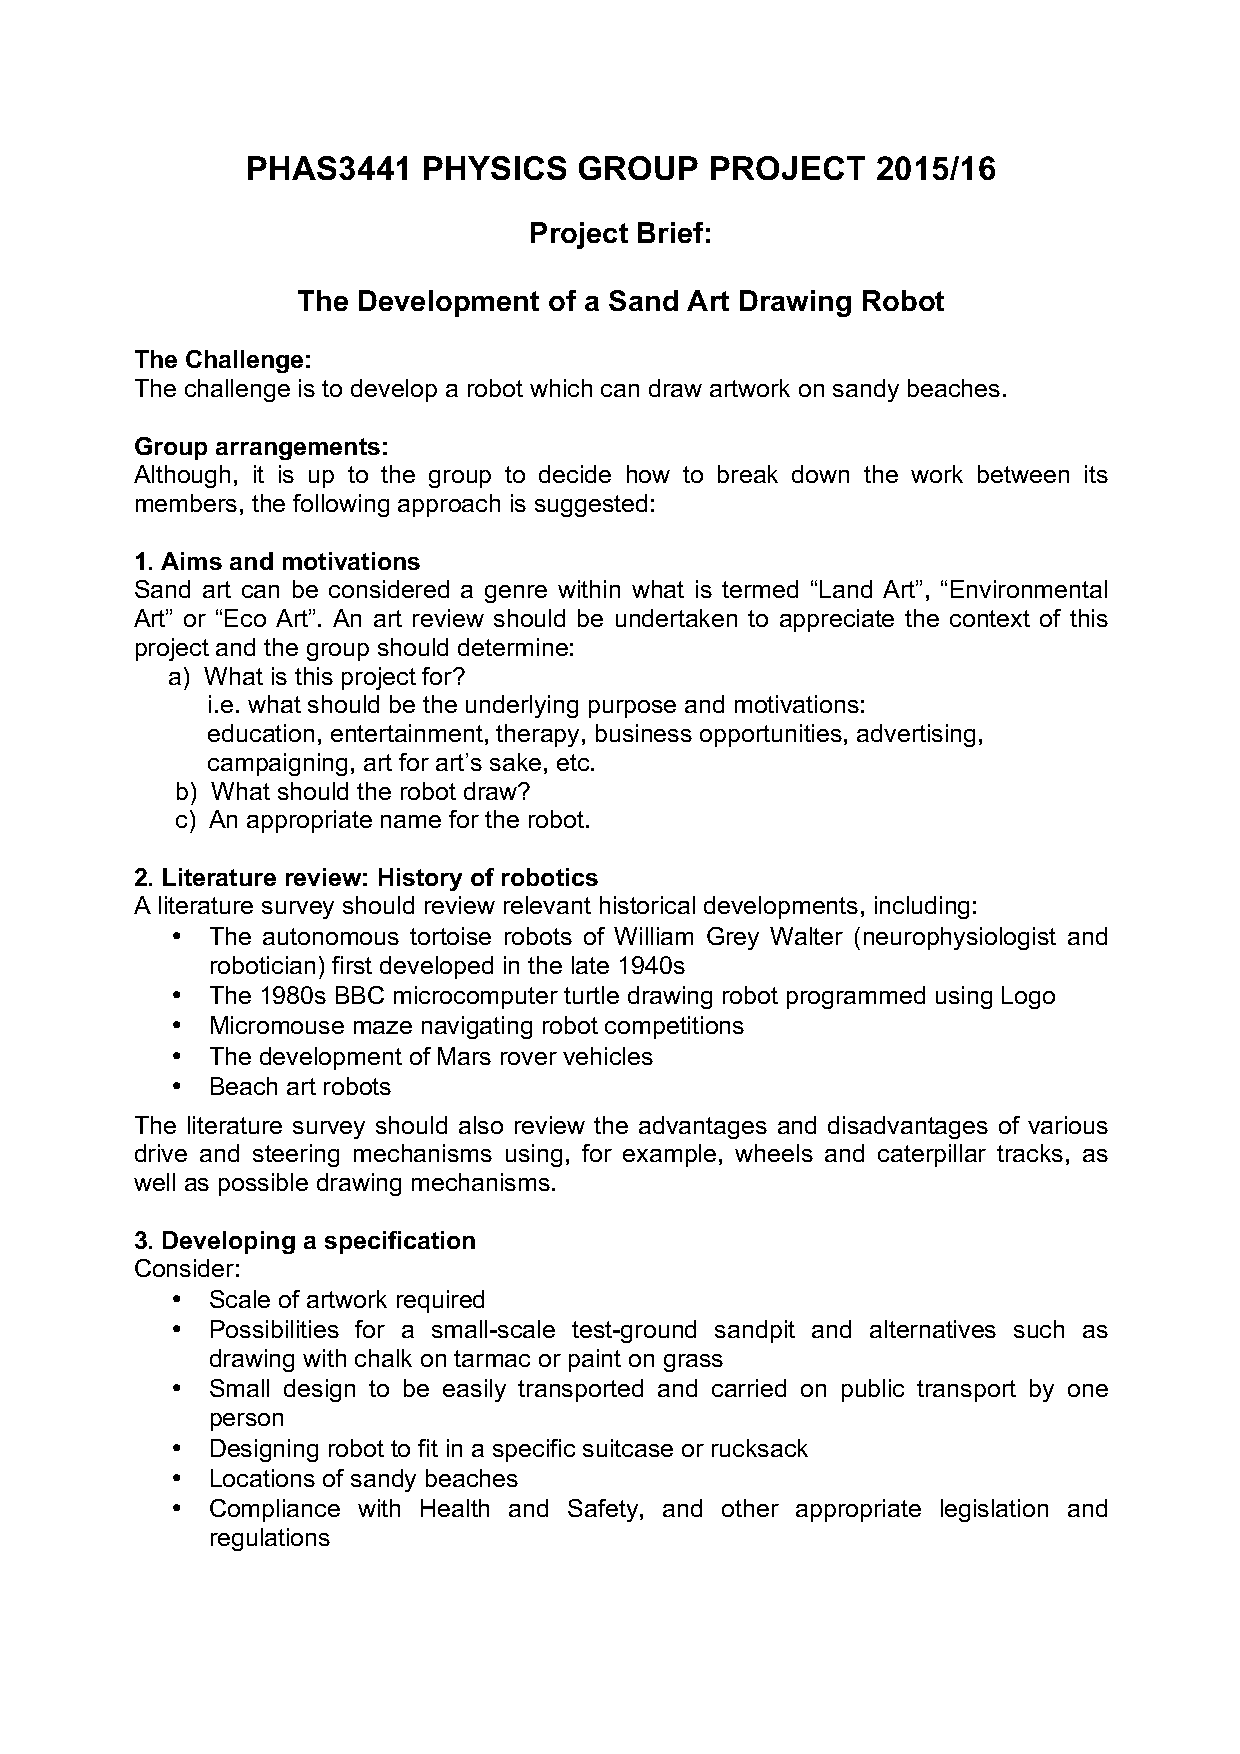
\includepdf[pages={-}]{../Files/project_brief.pdf}

\end{document}
